\documentclass{article}
\usepackage{graphicx} % Required for inserting images
\usepackage[english]{babel}
\usepackage{amsmath}
\usepackage{amsfonts}
\usepackage{amsthm}
\usepackage{amssymb}
\usepackage{physics}
\usepackage[mathscr]{euscript}
\let\euscr\mathscr \let\mathscr\relax
\usepackage[scr]{rsfso}
\newcommand{\powerset}{\raisebox{.15\baselineskip}{\Large\ensuremath{\wp}}}


\usepackage{mathtools}


\numberwithin{equation}{section}

\newcommand{\vah}[1]{\va{\hat{#1}}}
\newcommand{\vbh}[1]{\vb{\hat{#1}}}
\newcommand{\set}[1]{\{#1\}}
\newcommand{\FT}{\mathcal{F}}
\newcommand\perm[2][^n]{\prescript{#1\mkern-2.5mu}{}P_{#2}}
\newcommand\comb[2][^n]{\prescript{#1\mkern-0.5mu}{}C_{#2}}

\DeclareMathOperator{\spn}{span}

\makeatletter
\renewcommand*\env@matrix[1][*\c@MaxMatrixCols c]{%
  \hskip -\arraycolsep
  \let\@ifnextchar\new@ifnextchar
  \array{#1}}
\makeatother

\newtheorem{theorem}{Theorem}[section]
\newtheorem{corollary}{Corollary}[theorem]
\newtheorem{lemma}[theorem]{Lemma}

\title{PHYS 110A Quiz 1}
\author{Siyu Chen}
\date{Summer 2023}

\begin{document}

\maketitle

\begin{figure}[h]
\centering
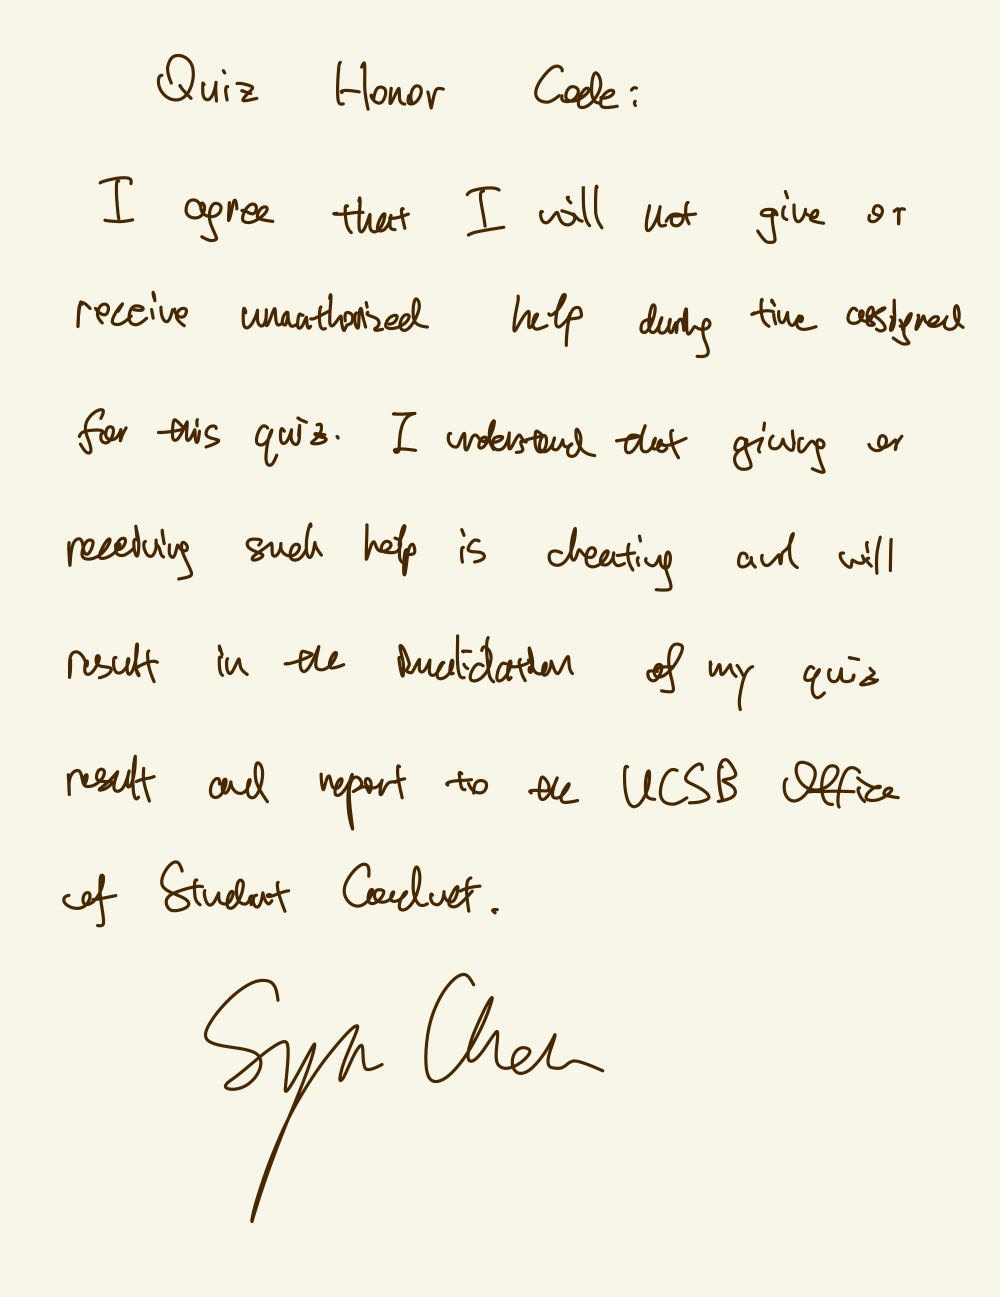
\includegraphics[width=0.8\textwidth]{quizzes/quiz honor code.jpg}
\caption{Signed Quiz Honor Code of Siyu Chen}
\end{figure}

\section{Problem 1}

Consider the expression for $A \cross B$, and $C \cross D$ with different indices for clarity:

\begin{equation}
    \begin{split}
        \vb{A} \cross \vb{B} &= \epsilon_{ijk} A_i B_j \vbh{e}_k \\
        \vb{C} \cross \vb{D} &= \epsilon_{lmn} C_l B_m \vbh{e}_n
    \end{split}
\end{equation}

Our equation has the form of the cross product of these two, which is:
\begin{equation}
    \epsilon_{ijk} \epsilon_{lmn} (A_i B_j \vbh{e}_k) \cdot ( C_l B_m \vbh{e}_n)
\end{equation}

Since $\vbh{e}_k \cdot \vbh{e}_n =  \delta_{kn}$, we have:

\begin{equation}
    \epsilon_{ijk} \epsilon_{lmk} A_i B_j C_l B_m 
\end{equation}

and evaluating the contraction between the two Levi-Civita symbols, we have:

\begin{equation}
    \epsilon_{ijk} \epsilon_{lmk} = \begin{vmatrix}
        \delta_{il} & \delta_{im} &  \delta_{ik} \\ \delta_{jl} & \delta_{jm} &  \delta_{jk} \\ \delta_kl & \delta_km &  \delta_kk
    \end{vmatrix} = \delta_{il} \delta_{jm} - \delta_{jl} \delta_{im}
\end{equation}

so our equation becomes:

\begin{equation}
    (\delta_{il} \delta_{jm} - \delta_{jl} \delta_{im}) A_i B_j C_l D_m = A_i C_i B_j D_j - A_i D_i B_j C_j = (\vb{A} \cdot \vb{C})(\vb{B} \cdot \vb{D}) - (\vb{A} \cdot \vb{D}) (\vb{B} \cdot \vb{C})
\end{equation}

and that is our correct equation.

\section{Problem 2}

Let $\vb{r} = x_i \vbh{e_i}$

\paragraph{(a) $\div \vb{r}$}

By the definition of divergence, we have:

\begin{equation}
    \begin{split}
        \div \vb{r} = (\partial_j \vbh{e_j}) \cdot (x_i \vbh{e_i}) = \partial_j x_i \vbh{e_i} \cdot \vbh{e_j}
    \end{split}
\end{equation}

Since $\vbh{e_i} \cdot \vbh{e_j} = \delta_{ij}$, we have:

\begin{equation}
     \div \vb{r} = \partial_i x_i = 3
\end{equation}

Since $\partial_1 x_1 = 1, \partial_2 x_2 = 1, \partial_3 x_3 = 1$.

\paragraph{(b) $\curl \vb{r}$}

Since, extending from part (a), we know that $\vb{r} = x_1 \vbh{e_1} + x_2 \vbh{e_2}+x_3 \vbh{e_3}$ and $\partial_1 x_1 = 1, \partial_2 x_1 = 0$, we can see that $\partial_i x_j = \delta_{ij}$ for our positional vector $\vb{r}$

\begin{equation}
    \begin{split}
        \curl \vb{r} &= (\partial_i \vbh{e}_i) \cross (x_j \vbh{e}_j) \\
        &= \partial_i x_j (\vbh{e_i \cross e_j}) \\
        &= \partial_i x_j \vbh{e}_k \epsilon_{ijk} = \delta_{ij} \vbh{e}_k \epsilon_{ijk} = 0
    \end{split}
\end{equation}

\paragraph{(c) $\grad r$}

Since $r = (x_1 + x_2 + x_3)$

\end{document}